We show related works in format of directed graph where node represents a work and edge represents a citation
between two works.
For example, the node 12 (current manuscript) cites the manuscripts 7 and 8.
Nodes of the graph are
\begin{itemize}
    \item {\Large \textcircled{\normalsize 12}} is this manuscript
    \item {\Large \textcircled{\normalsize 7}} is \textit{A study on partial dynamic equation on time scales involving derivatives
    of polynomials}~\cite{kolosov2016study}
    \item {\Large \textcircled{\normalsize 8}} is \textit{106.37 An unusual identity for odd-powers}~\cite{kolosov2022106}
    \item {\Large \textcircled{\normalsize 9}} is \textit{Another approach to get derivative of odd-power}~\cite{kolosov2023another}
    \item {\Large \textcircled{\normalsize B}} is \textit{A two-sided Faulhaber-like formula involving Bernoulli polynomials}~\cite{barbero2020two}
    \item {\Large \textcircled{\normalsize 10}} is \textit{Polynomial identity involving Binomial Theorem and Faulhaber's formula}~\cite{kolosov2023polynomial}
    \item {\Large \textcircled{\normalsize 11}} is \textit{Finding the derivative of polynomials via double limit}~\cite{kolosov_2024_10575485}
    \item {\Large \textcircled{\normalsize 6}} is \textit{On the link between binomial theorem and discrete convolution}~\cite{kolosov2016link}
\end{itemize}
\begin{figure}[H]
    \centering
    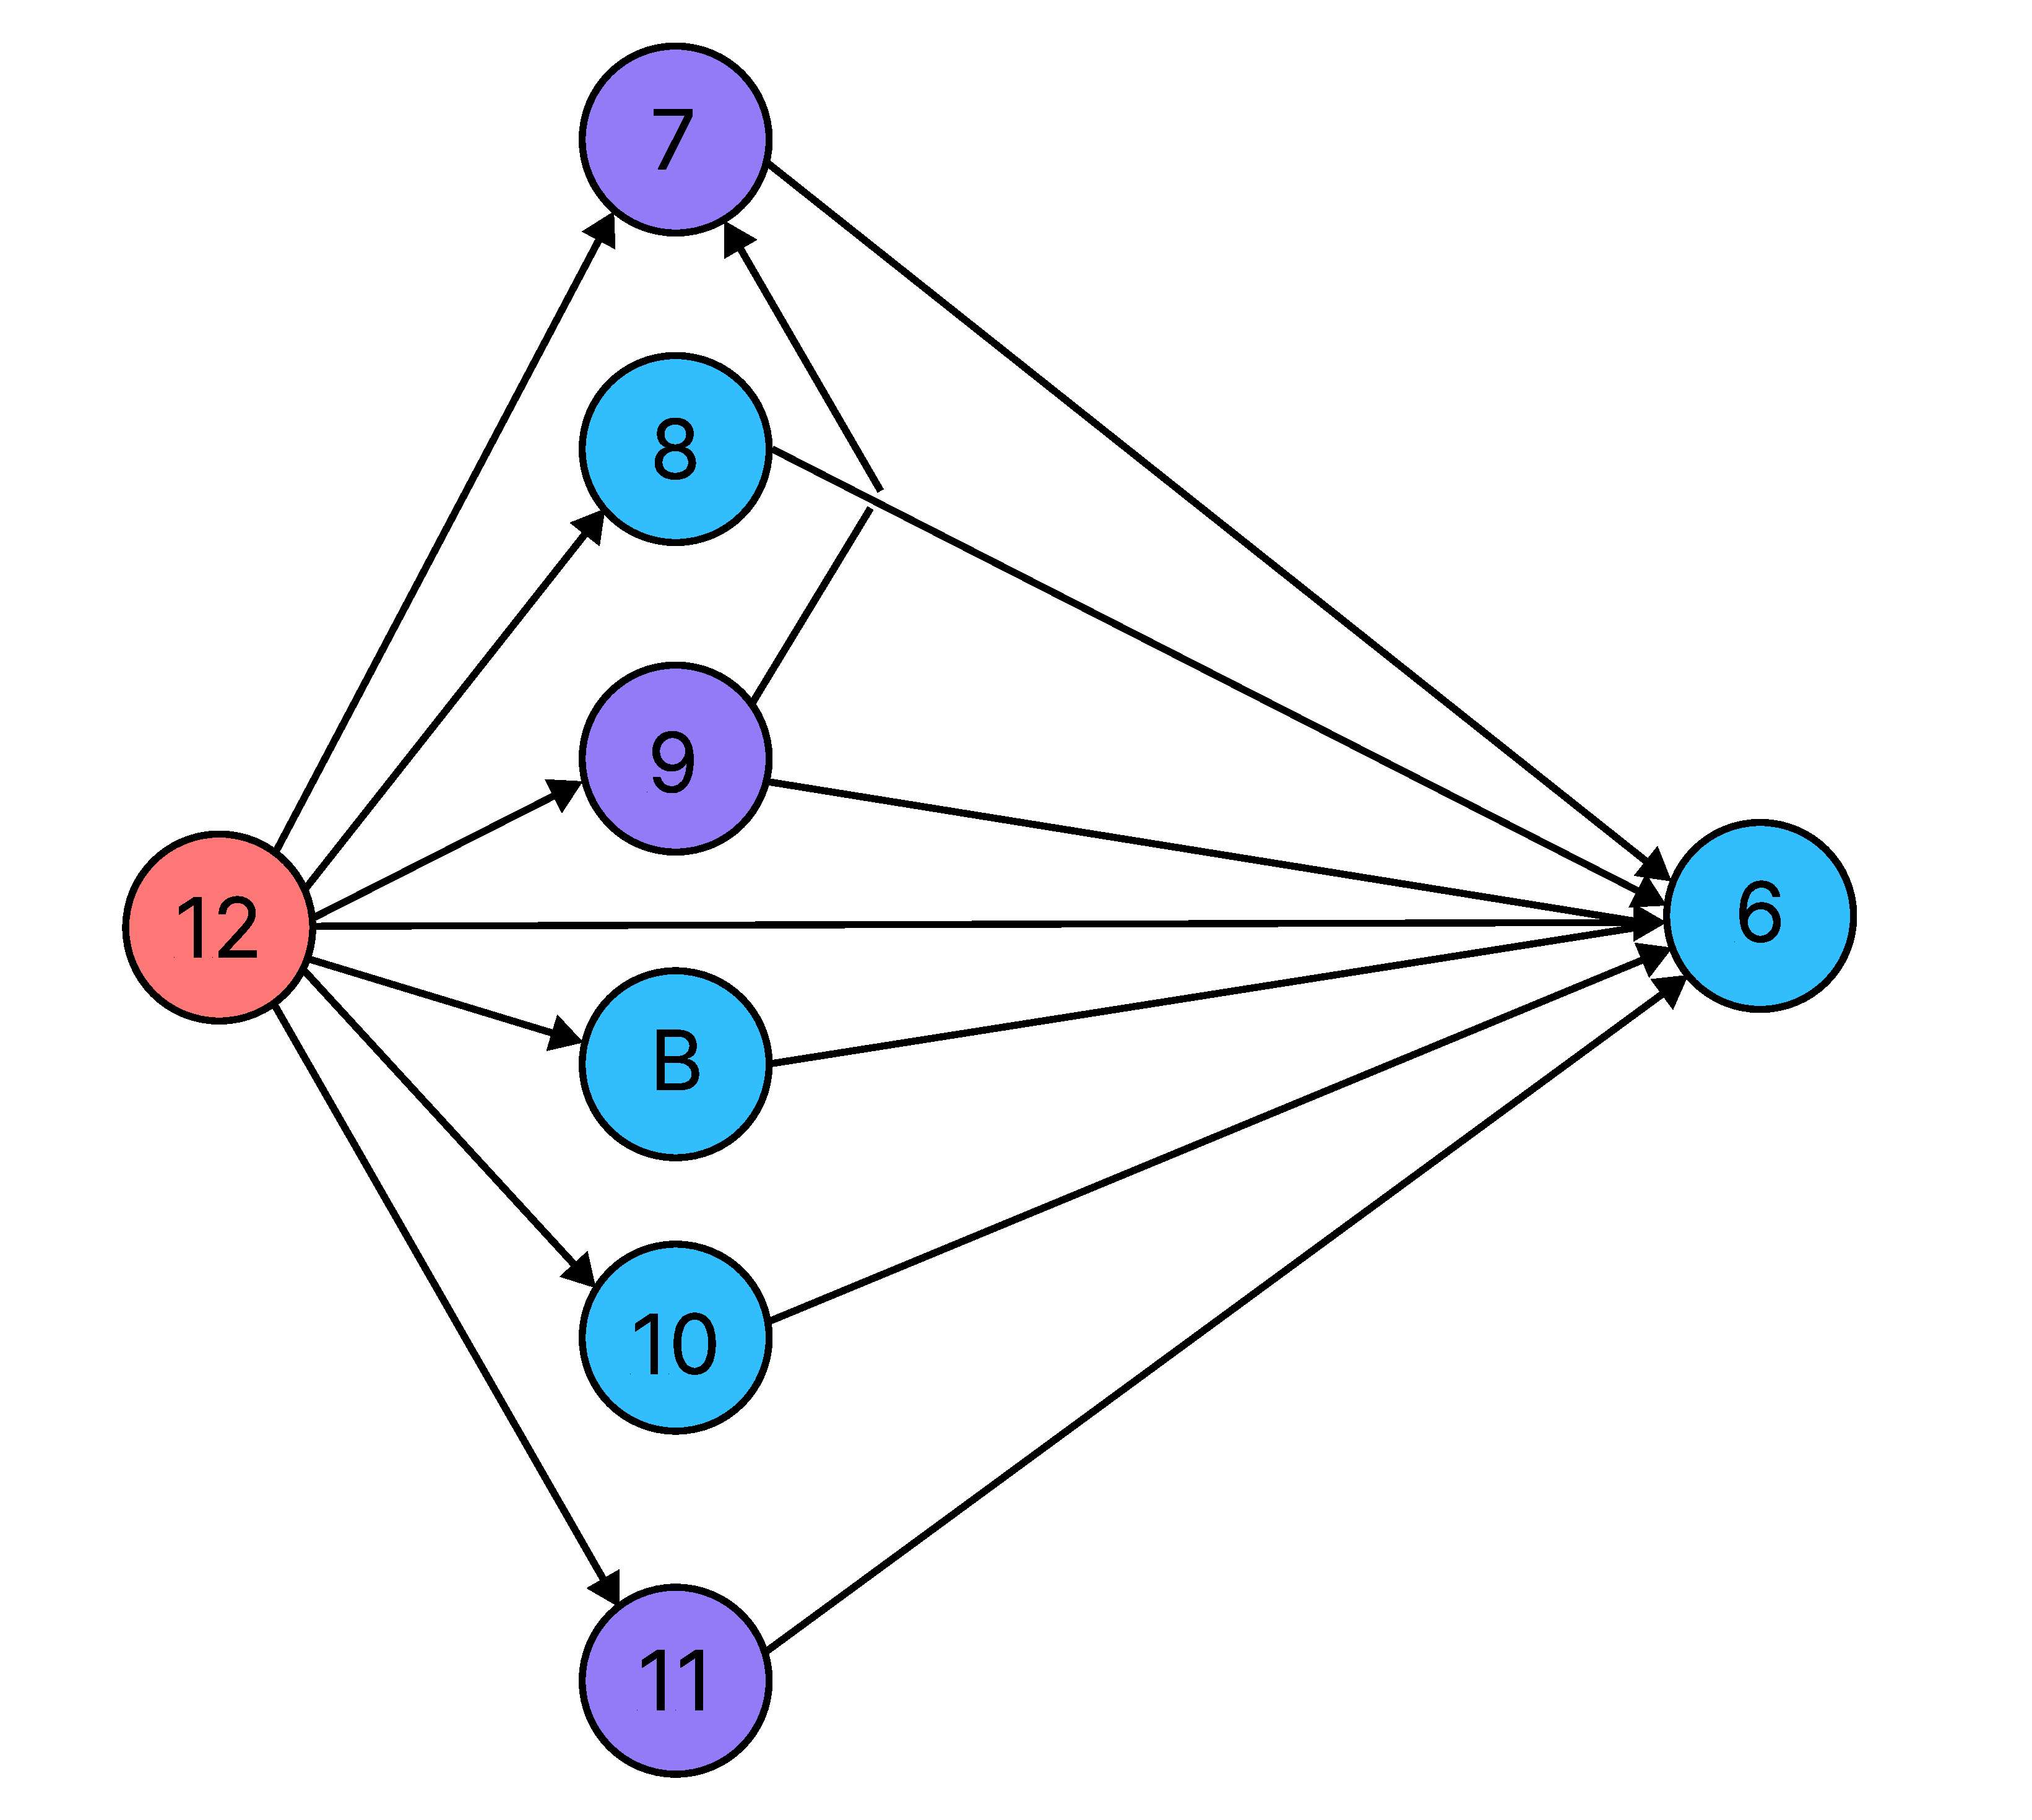
\includegraphics[width=1\textwidth]{images/realated_works_graph}
    ~\caption{Related works graph.}\label{fig:related-works-graph}
\end{figure}
\begin{itemize}
    \item {\Large \textcircled{\normalsize 12}} This manuscript
    \item {\Large \textcircled{\normalsize 6}}
    In \textit{On the link between binomial theorem and discrete convolution}~\cite{kolosov2016link}:
    Let $\mathbf{P}^{m}_{b}(x)$ be a $2m+1$-degree polynomial in $x$ and $b \in \mathbb{R}$
    \[
        \mathbf{P}^{m}_{b}(x) = \sum_{k=0}^{b-1} \sum_{r=0}^{m} \mathbf{A}_{m,r} k^r (x-k)^r
    \]
    where $\mathbf{A}_{m,r}$ are real coefficients.
    In this manuscript, we introduce the polynomial $\mathbf{P}^{m}_{b}(x)$ and study its properties,
    establishing a polynomial identity for odd-powers in terms of this polynomial.
    Based on mentioned polynomial identity for odd-powers,
    we explore the connection between the Binomial theorem and discrete convolution of odd-powers,
    further extending this relation to the multinomial case.
    All findings are verified using Mathematica programs.
    \item {\Large \textcircled{\normalsize 7}}
    In \textit{A study on partial dynamic equation on time scales involving derivatives
    of polynomials}~\cite{kolosov2016study}:
    Extends the main results of {\Large \textcircled{\normalsize 6}} deriving and discussing
    an identity that connects the timescale derivative of odd-powered polynomial
    with partial derivatives of polynomial $\polynomialP{m}{b}{x}$ evaluated in particular points.
    For every $t\in\mathbb{T}_1$ and $(x,b) \in \Lambda^2$
    \[
        \frac{\Delta x^{2m+1}}{\Delta x}(t) =
        \frac{\partial P(m,b,x)}{\Delta x} (m, \sigma(t), t) +
        \frac{\partial P(m,b,x)}{\Delta b} (m, t, t)
    \]
    such that $\sigma(t) > t$ is forward jump operator.
    In addition, we discuss various derivative operators in the context of the partial cases of above equation,
    We show finite difference, classical derivative, $q-$derivative, $q-$power derivative on behalf of it.
    \item {\Large \textcircled{\normalsize 8}}
    In \textit{106.37 An unusual identity for odd-powers}~\cite{kolosov2022106}:
    Explores and proves the partial case of {\Large \textcircled{\normalsize 6}}
    that is the polynomial identity for odd-powers
    \[
        n^{2m+1} = \sum_{k=1}^{n} \sum_{r=0}^{m} \mathbf{A}_{m,r} k^r (n-k)^r
    \]
    \item {\Large \textcircled{\normalsize 9}}
    In \textit{Another approach to get derivative of odd-power}~\cite{kolosov2023another}:
    Extends the results of {\Large \textcircled{\normalsize 6}} by providing a relation in terms of partial differential equations such that
    ordinary derivative of odd-power $2m+1$ can be reached in terms of partial derivative of the polynomial $\polynomialP{m}{b}{x}$.
    Let be a fixed point $v\in \mathbb{N}$, then ordinary derivative $\frac{d}{dx} g_v (u)$ of the odd-power function $g_v(x) = x^{2v + 1}$
    evaluate in point $u\in\mathbb{R}$ equals to partial derivative $(f_{v})^{'}_{x} (u, u)$ evaluate in point $(u, u)$ plus
    partial derivative $(f_{v})^{'}_{z} (u, u)$ evaluate in point $(u, u)$
    \begin{equation}
        \frac{d}{dx} g_v (u) = (f_{v})^{'}_{x} (u, u) + (f_{v})^{'}_{z} (u, u)
        \label{eq:odd-exponential-identity}
    \end{equation}
    where $f_{y} (x, z) = \sum_{k=1}^{z} \sum_{r=0}^{y} \coeffA{y}{r} k^r (x-k)^r = \polynomialP{y}{z}{x}$.
%    \item {\Large \textcircled{\normalsize 11}}
%    In \textit{Finding the derivative of polynomials via double limit}~\cite{kolosov_2024_10575485}:
%    Applies the results {\Large \textcircled{\normalsize 6}} by providing
%    another perspective of ordinary derivatives of polynomials allowing expressing
%    them via a double limit, because
%    \begin{align*}
%        \lim_{h \to 0} \polynomialP{m}{x+h}{x} = x^{2m+1}
%    \end{align*}
    \item {\Large \textcircled{\normalsize B}}
    In \textit{A two-sided Faulhaber-like formula involving Bernoulli polynomials}~\cite{barbero2020two}:
    Based on equation~\eqref{eq:equation7}, the authors give a new identity involving
    Bernoulli polynomials and combinatorial numbers that provides,
    in particular, the Faulhaber-like formula for sums of the form $1^m(n-1)^m + 2^m (n -2)^m + \cdots + (n - 1)^m 1^m$
    for positive integers $m$ and $n$.
    \item {\Large \textcircled{\normalsize 10}}
    In \textit{Polynomial identity involving Binomial Theorem and Faulhaber's formula}~\cite{kolosov2023polynomial}:
    proves that
    for every $n\geq 1, \; n,m\in\mathbb{N}$
    there are coefficients $\mathbf{A}_{m,0}, \mathbf{A}_{m,1}, \ldots, \mathbf{A}_{m,m}$ such that
    the polynomial identity holds
    \[
        n^{2m+1} = \sum_{k=1}^{n} \mathbf{A}_{m,0} k^0 (n-k)^0 + \mathbf{A}_{m,1}(n-k)^1
        + \cdots + \mathbf{A}_{m,m} k^m (n-k)^m
    \]
    which is a direct consequence of the definition of $\polynomialP{m}{b}{x}$ given in {\Large \textcircled{\normalsize 6}},
    reached by utilizing Binomial theorem and Faulhaber's formula.
    \item {\Large \textcircled{\normalsize 11}}
    In \textit{Finding the derivative of polynomials via double limit}~\cite{kolosov_2024_10575485}:
    By applying the results of {\Large \textcircled{\normalsize 6}} provides
    another perspective of ordinary derivatives of polynomials allowing expressing
    them via a double limit, because
    \begin{align*}
        \lim_{h \to 0} \polynomialP{m}{x+h}{x} = x^{2m+1}
    \end{align*}
%    \item {\Large \textcircled{\normalsize B}}
%    In \textit{A two-sided Faulhaber-like formula involving Bernoulli polynomials}~\cite{barbero2020two}:
%    Based on~\eqref{eq:equation7}, the authors give a new identity involving
%    Bernoulli polynomials and combinatorial numbers that provides,
%    in particular, the Faulhaber-like formula for sums of the form $1^m(n-1)^m + 2^m (n -2)^m + \cdots + (n - 1)^m 1^m$
%    for positive integers $m$ and $n$.
%    \item {\Large \textcircled{\normalsize 6}}
%    In \textit{On the link between binomial theorem and discrete convolution}~\cite{kolosov2016link}:
%    Let $\mathbf{P}^{m}_{b}(x)$ be a $2m+1$-degree polynomial in $x$ and $b \in \mathbb{R}$
%    \[
%        \mathbf{P}^{m}_{b}(x) = \sum_{k=0}^{b-1} \sum_{r=0}^{m} \mathbf{A}_{m,r} k^r (x-k)^r
%    \]
%    where $\mathbf{A}_{m,r}$ are real coefficients.
%    In this manuscript, we introduce the polynomial $\mathbf{P}^{m}_{b}(x)$ and study its properties,
%    establishing a polynomial identity for odd-powers in terms of this polynomial.
%    Based on mentioned polynomial identity for odd-powers,
%    we explore the connection between the Binomial theorem and discrete convolution of odd-powers,
%    further extending this relation to the multinomial case.
%    All findings are verified using Mathematica programs.
    \item Three sequences were contributed to the
    OEIS~\cite{kolosov2018coefficientspolynomial1, kolosov2018coefficientspolynomial2, kolosov2018coefficientspolynomial3}
    showing the coefficients of the polynomial $\polynomialP{m}{b}{x}$ having fixed points $m,b$ while $x\in\mathbb{R}$.
    \item OEIS sequences such that row sums give odd-powers~\cite{kolosov2017third, kolosov2018fifth, kolosov2018seventh}.
    \item OEIS sequences related to the coefficients $\coeffA{m}{r}$~\cite{kolosov2018numerator, kolosov2018denominator}.
\end{itemize}
The indexes of the related works graph are same that are on the website
\begin{center}
    \href{https://kolosovpetro.github.io/math/}{\texttt{kolosovpetro.github.io/math}}
\end{center}
